%%%%%%%%%%%%%%%%%%%%%%%%%%%%%%%%%%%%%%%%%%%%%%%%%%%%%%%%%%%%%%%%%%%%%%%%%%%%%%%
%% LaTeX-Vorlage für Abschlussarbeiten (Koma-Script)                         %%
%% (TH Köln -Campus Gummersbach, Fak. 10)                                    %%
%%                                                                           %%
%% Gemäß dem Merkblatt zur Anfertigung von Projekt-, Bachelor-, Master- und  %%
%% Diplomarbeiten der Fakultät 10 von Frau Prof. Dr. Halfmann &              %%
%% Herr Prof. Dr. Rühmann (Version vom 27.01.2008)                           %%
%%                                                                           %%
%% LIZENZ:                                                                   %%
%% Diese Vorlage darf nicht kommerziell verbreitet                           %%
%% werden. Eine nicht-kommerzielle Weitergabe ist                            %%
%% gestattet.                                                                %%
%%                                                                           %%
%% Von Ludger Schönfeld, M. Sc.,                                             %%
%% 2015-2017 (Stand: 05.04.17)                                               %%
%%%%%%%%%%%%%%%%%%%%%%%%%%%%%%%%%%%%%%%%%%%%%%%%%%%%%%%%%%%%%%%%%%%%%%%%%%%%%%%

\documentclass[a4paper,fontsize=12pt,abstract=true, toc=nolistof,headsepline=true,footsepline=true]{scrartcl}
%%INFO: Dokumenteinstellungen
% - fontsize: Schriftgröße (hier jede beliebige, Standard: 11pt)
% - abstract: Überschrift zum Abstract ein-/abschalten (Werte: true/false)
% - toc: Gestalt des Inhaltsverzeichnisses beeinflussen (s. KOMA-Script-Guide).
%   Wert "listof/nolistof" => Verzeichnisse von Tabellen & Abbildungen werden unnummeriert ins Inhaltsverzeichnis aufgenommen bzw. nicht ins Inhaltsverzeichnis aufgenommen.
% - headsepline: Ein-/Ausschalten einer Linie in der Kopfzeile.
% - footsepline: Ein-/Ausschalten einer Linie in der Fusszeile.
%

\usepackage[ngerman]{babel}
\usepackage[T1]{fontenc} % Schriftkodierung (Für Sonderzeichen u.a.)
\usepackage[utf8]{inputenc} % Für die direkte Eingabe von Umlauten im Editor u.a. - ACHTUNG: Kodierung muss mit der Zeichenkodierung im Editor übereinstimmen!
\usepackage{microtype} % Verbesserter Randausgleich
\usepackage{lmodern}
\usepackage{parskip}

%% Paket für Beispiel-Text (Pseudo-Latein)
% => Befehl (Bsp.): \lipsum[2-4]
\usepackage{lipsum}

%% Zeilenabstand setzen
\usepackage[onehalfspacing]{setspace}
% INFO: Zeilenabstand setzen:
%
% Befehle:
% - \singlespacing  => 1-zeilig (Standard)
% - \onehalfspacing => 1,5-zeilig
% - \doublespacing  => 2-zeilig

%% Satzspiegel einrichten
\usepackage[left=3cm,right=2cm,top=1.5cm,bottom=1cm,
    textheight=245mm,textwidth=160mm,includeheadfoot,headsep=1cm,
    footskip=1cm,headheight=14.599pt]{geometry} % Einrichtung der Seite
% KOMA-Script bietet das Paket "typearea". Dieses berechnet Ihnen eine optimale Seiteneinstellung. Bei diesem Paket haben Sie allerdings nicht so viele Einstellungsmöglichkeiten.

%% Einstellungen für Marginalien (Beispiel)
%%(Randkommentierung mit \marginpar{Text})
%\newcommand\mpar[1]{\marginpar {\flushleft\sffamily\small #1}}
%\setlength{\marginparwidth}{3cm}

%% Einbinden von Graphiken
\usepackage{graphicx}
\usepackage{epstopdf} % Umwandlung EPS-Bilder => PDF, sodass diese auch mithilfe des Tools "pdflatex" eingebunden werden können
% Unterstreichen von Text
\usepackage[normalem]{ulem} % Befehl: \uline{}

%% Pakete für Tabellen
\usepackage{tabularx} % Einfache Tabellen
\usepackage{longtable} % Tabellen als Gleitobjekte (für die Aufteilung bei langen Tabellen über mehrere Seiten)
\usepackage{multirow} % Verbinden von Zeilen innerhalb einer Tabelle mit \multirow{anzahl}{*}{Text}
\usepackage{pbox}

% (Zusatz-)Pakete für Formeln
\usepackage{amsmath}
\usepackage{amsthm}
\usepackage{amsfonts}

% Farbboxen (für die Merkkästen in dieser Vorlage):
\usepackage{tcolorbox}
\tcbset{colback=white,colframe=orange,
    fonttitle=\bfseries}

%% Autom. Literaturverzeichnisse mit dem Paket 'biblatex'":
\usepackage{biblatex}
\addbibresource{bib/sources.bib}

\usepackage[colorlinks,pdfpagelabels,pdfstartview=FitH,
    bookmarksopen=true,bookmarksnumbered=true,linkcolor=black,
    plainpages=false,hypertexnames=false,citecolor=black]{hyperref} % Für Verlinkungen
% INFO: Verlinkungen mit dem hyperref-Paket:
%
% Die Angabe von URLs mit dem Befehl \url{} erlaubt einen
% gesonderten Umgang mit Weblinks. Denn die Links werden verlinkt.
% Auch erfolgt automatisch am Zeilenende ein Umbruch des Links.
% Es ist auch nicht erforderlich, Sonderzeichen in der URL manuell zu
% entschärfen.
%
% TIPP: Sollte ein Umbruch bei einem Link nicht automatisch erfolgen, so kann
% das daran liegen, dass ein/mehrere Zeichen zusätzlich angegeben werden müssen,
% an dem der Link umbrochen werden kann.
% => Siehe Paket "breakurl"

\usepackage{pdfpages}

\usepackage{array,etoolbox}
\usepackage{csquotes}
\preto\tabular{\setcounter{magicrownumbers}{0}}
\newcounter{magicrownumbers}
\newcommand\rownumber{\stepcounter{magicrownumbers}\arabic{magicrownumbers}}

\newcommand{\newlineparagraph}[1]{\paragraph{#1}\mbox{}\\}

\begin{document}
    \pagestyle{empty}
\begin{titlepage}
    
\includegraphics[scale=1.0]{assets/logo_TH-Koeln_CMYK_22pt}\\
    \begin{center}
        \large
        Technische Hochschule Köln\\
        Fakultät für Informatik und Ingenieurwissenschaften\\
        \vspace{1cm}
        \large
        \textsc{Praxisprojekt}\\
        \vspace{1cm}
        \huge
        Praktische Evaluation des Frameworks\\
        Laravel Nova am Beispiel einer Anwendung\\
        zur Verwaltung und Auswertung von\\
        Radiosondenaufstiegen\\
        \vspace{1cm}
        \large
        vorgelegt an der TH Köln\\
        Campus Gummersbach\\
        im Studiengang\\
        Medieninformatik\\
        \vspace{1cm}
        ausgearbeitet von:\\
        \textsc{Niklas Canisius}\\
        (Matrikelnummer: 11110023)\\
        \vspace{1cm}
        \begin{tabular}{ll}
            \textbf{Betreuer:} & Prof.\ Dr. Christian Kohls \\
        \end{tabular}
        \vspace{1cm}
        \\Gummersbach, den \today
    \end{center}
\end{titlepage}

    \newpage


\section*{Sperrvermerk}
Das vorliegende Dokument beinhaltet vertrauliche Daten der Firma Graw Radiosondes GmbH \& Co. KG sowie der Kiwis \& Brownies GbR.
Es darf nur von berechtigten Personen innerhalb Ihrer dienstlichen Verpflichtungen eingesehen werden.

Eine Veröffentlichung und Vervielfältigung – auch in Teilen – ist untersagt.
Dritten darf dieses Dokument nur mit der ausdrücklichen Genehmigung des Verfassers und beider Unternehmen zugänglich gemacht werden.

Der Sperrvermerk gilt für ein Jahr ab dem \today.

    \newpage


\section*{Kurzzusammenfassung}
Radiosonden sind Instrumente zur Messung meteorologischer bzw.\ aerologischer Daten aus der Erdatmosphäre.
Für die Verwaltung und Auswertung von mehreren Bodenstationen und deren Radiosondenaufstiegen wird eine webbasierte Software entwickelt.
Ziel dieser Arbeit ist die Konzeption und Implementierung eines ersten lauffähigen, sowie produktiv nutzbaren Prototypen der Software.
Außerdem sollen zwei Hostingvarianten, Cloud based und On-Premises, umgesetzt werden.

Im Rahmen dieser praktischen Arbeit wird evaluiert, welche Vor- und Nachteile der Einsatz eines Admin-Panel Frameworks, am konkreten Beispiel von Laravel Nova, bietet.
Zusätzlich wird ein Vergleich zu ähnlichen Technologien, im methodischen Rahmen einer kurzen Nutzwertanalyse, gezogen.

Laravel Nova überzeugt durch stark gesteigerte Produktivität während der Implementierung.
In puncto Anpassbarkeit müssen dafür jedoch einige Einschränkungen in Kauf genommen werden.
Der Verglich mit ähnlichen Frameworks zeigt, dass es möglicherweise besser geeignete Kandidaten gibt.


    \newpage
    \renewcommand{\contentsname}{Inhaltsverzeichnis}
    \tableofcontents
    \newpage

    \pagestyle{headings} % Kopf- und Fußzeilen aktivieren
    \pagenumbering{arabic} % Seitennummerierung: arabische Zahlen

    \newpage


\section{Einleitung}

\subsection{Motivation}

\subsection{Projektstruktur und Anforderungen}

\subsection{Forschungsfrage}

    \section{Grundlagen}

\subsection{Marktrecherche}
Der größere Konkurrent bietet für seine Kunden, die ganze Messnetzwerke betreuen, bereits eine Lösung an.
Der sogenannte \enquote{Vaisala Observation Network Manager}\cite{observation-network-manager} bietet einen ähnlichen inhaltlichen Umfang.
Die Implementierung basiert ebenfalls auf Webtechnologien und bestätigt damit in diesem Punkt den Ansatz von GRAW.

\subsection{Methodik und Vorgehensmodelle}
In kurzer Projektzeit wird ein umfangreicher und lauffähiger Prototyp bzw.\ ein MVP erstellt.
Für eine langfristige Planung ist daher keine Zeit und so wird auf das Entwicklungsmodell XP (Extreme Programming) gesetzt.
Dafür werden im Projektverlauf die bei XP üblichen fünf Werte und die 14 Prinzipien (Vergleiche~\cite{agile-prozesse}) berücksichtigt und auf das vorliegende Projekt angewendet.

Im Anschluss an die Implementierung der Software wird, zusätzlich zu den praktischen Erfahrungswerten durch die Implementierung, eine Nutzwertanalyse durchgeführt.
Methodisch wird sich dabei an einem Praxisleitfaden~\cite{scoring-und-nutzwertanalysen} orientiert.
Ziel dieses Methodeneinsatzes ist es, das abschließende Fazit rationaler zu gestalten.
Analyseinhalt ist ein kurzer Vergleich von Nova mit anderen populären Laravel Admin Panels (Vergleiche~\cite{the-guide-to-laravel-admin-panels}), die Auswahl und Gewichtung von Entscheidungskriterien sowie das daraus resultierende Scoring.

\subsection{Technische Entwurfsmuster}

\subsubsection{Model View Controller}
MVC ist ein etabliertes Entwurfsmuster für Benutzerinterfaces.
Durch eine Zuständigkeitstrennung werden Wartungen einfacher und können besser auf unterschiedliche Entwickler aufgeteilt werden.
Das Model ist nur zuständig für Daten und Business Logic, die View hingegen nur für die Darstellung der Inhalte (\ref{fig:mvc})).
Der Controller ist das Bindeglied, indem er Daten und Befehle zwischen den anderen beiden Bereichen routet.
(Vergleiche~\cite{mdn-glossary-mvc})

\begin{figure}[h!]
    \centering
    \caption{Model View Controller}
    \label{fig:mvc}
    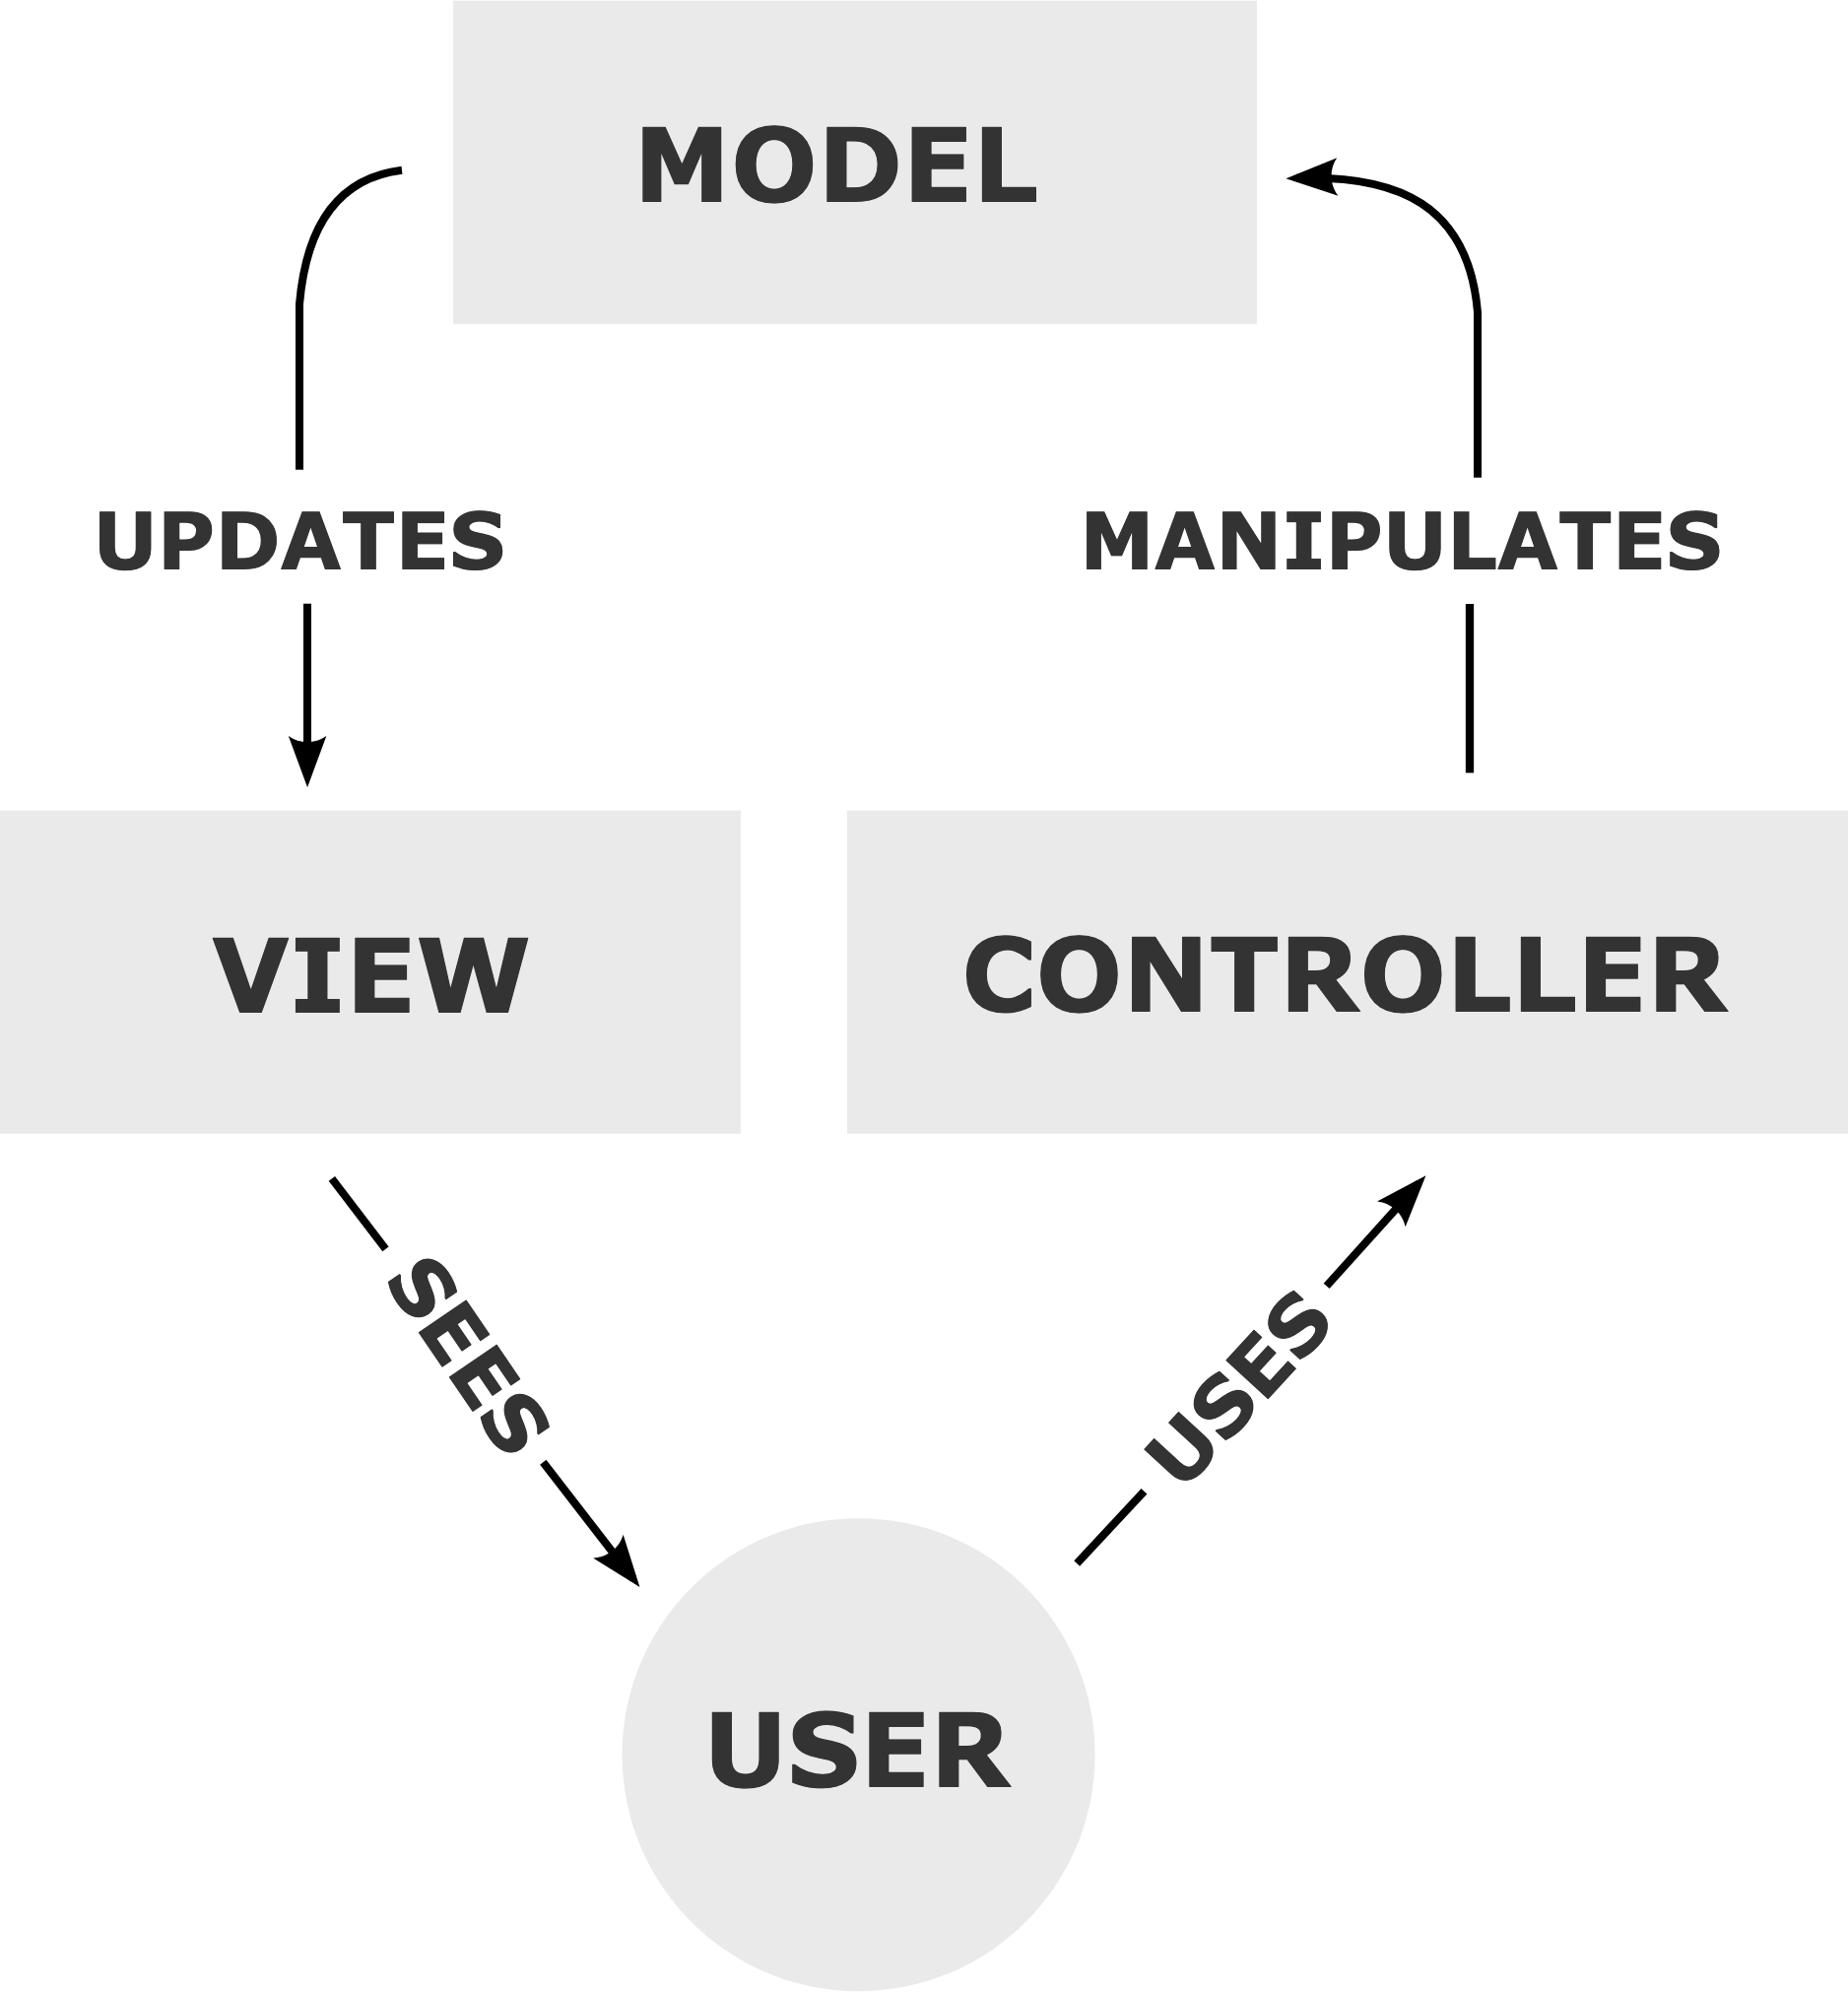
\includegraphics[scale=0.15]{assets/wikipedia_mvc_process}
\end{figure}

\newpage

\subsection{Technische Frameworks}

\subsubsection{Laravel}
Laravel ist ein kostenloses und quelloffenes Framework für die Erstellung moderner PHP Anwendungen.
Es bietet ein umfangreiches Toolset und eine umfangreiche Dokumentation, sowie ein großes Ecosystem weiterer Funktionsbibliotheken und passenden Services.
Laravel bietet eine MVC Architektur, eingebaute Security Features, eine Templating Engine, eine ORM (Object Relational Mapping) Library und vieles mehr.
In den letzten Jahren gewann es schnell an Popularität.
(Vergleiche~\cite{what-is-laravel})

\subsubsection{Laravel Nova}
Um Entwickler dabei zu unterstützen, besonders effizient und einfach, Administrationsinterfaces für Laravel Anwendungen zu entwickeln, wurde ein kostenpflichtiges first-party Framework entwickelt und veröffentlicht (Vergleiche ~\cite{laravel-nova}).
Oftmals haben Laravel Anwendungen eine öffentliche Website, eine API (Programmierschnittstelle) und einen Administrationsbereich für die Verwaltung der Daten (Vergleiche~\cite{laravel-up-and-running}).
Mit Laravel selbst lässt sich sehr gut eine API abdecken, ebenso ist es für öffentliche Websites designt.
Laravel Nova setzt also genau in dem Bereich an, den Entwickler in der Regel individuell aufbauen.

Für Datengetriebene Verwaltungsanwendungen üblich, und auch grundsätzlich durch Laravel vorbereitet, ist eine MVC Architektur.
Durch Nova bleibt allerdings lediglich die Definition des Models, inklusive der Datenbankmigrationen, allerdings fällt die übliche Programmlogik für Controller und View weg.
Stattdessen werden Ressourcen mit Feldern definiert, die je einem Model zugeordnet werden.
Dadurch lässt sich mit deutlich weniger Code, gegenüber einer individuellen Implementierung, die Verwaltung unterschiedlicher Ressourcen aufbauen.

    \section{Analyse}

\subsection{Problemraum und Anforderungen}
Für den Empfang von Messdaten und die korrekte Startvorbereitung benötigt eine Radiosonde von GRAW auch immer eine Bodenstation.
Auf Bodenstationen läuft unter Windows die Software \enquote{GRAWMET}\cite{grawmet}, welche die Daten der Sonde empfängt, weiterverarbeitet und auswertet.
Um vergangene Flüge auszuwerten und zu überwachen ist daher immer der Zugang zum Bodenstationscomputer notwendig.
Eine zentrale und einfache Auswertung mehrerer Stationen durch Nutzer an verschiedenen Orten mit verschiedenen Endgeräten ist aktuell kaum möglich.
Es gibt für diese Anforderungen bereits eine experimentelle Anwendung \enquote{GRAWgo}\cite{grawgo}, welche aufgrund ihrer Architektur kein On-Premises Hosting unterstützt und nur auf Mobilgeräten lauffähig ist.
GRAWgo hat es, vermutlich aufgrund seiner sehr eingeschränkten Nutzbarkeit, bisher nicht in einen produktiven Betrieb im Bereich von größeren Messnetzen geschafft und ist dafür auch aktuell nicht konzipiert.

Diese Probleme soll durch eine neue Architektur, bzw.\ eine ergänzende Software namens \enquote{Sounding Console}, gelöst werden.
Der Zugang zu den erfassten Daten und Auswertungen soll vereinfacht werden und von verschiedenen Orten aus möglich sein.
An dieser Problemstelle setzt die Sounding Console an und soll die sich daraus ergebenden Anforderungen erfüllen.

Grundsätzlich wurden durch den Auftraggeber Anforderungen im Rahmen eines Lastenheftes (\ref{subsec:lastenheft}) kommuniziert, diese wurden teilweise, nach technischer Einordnung durch den Verfasser dieser Arbeit, angepasst und ergänzt.
Anschließend wurde durch die auftragnehmende Agentur ein Angebot (\ref{subsec:angebot}) erstellt.
Nach Auftragseingang wurden konkretere Anforderungen und daraus resultierende Aufgaben durch den Entwickler, im sogenannten Leistungspaket (\ref{subsec:leistungspaket}), festgelegt.
Teilweise wurden in diesem Prozess offene Fragen mit dem Auftraggeber geklärt.

Im folgenden sind die Anforderungen gelistet, die die neue Software erfüllen soll.
Eine ausführlichere Darstellung findet sich im Anhang dieser Arbeit.
\newpage

\subsubsection{Inhaltliche Anforderungen}
Die inhaltlichen Anforderungen wurden überwiegend seitens des Auftraggebers erarbeitet, ergaben sich aber auch teilweise erst auf konkrete Rückfragen im Entwicklungsprozess.
\begin{itemize}
    \item Administratoren müssen Nutzern den Zugriff ermöglichen können und diesen durch eine Rollenzuweisung mit unterschiedlichen Zugriffsrechten weiter einschränken können.
    \item Im System müssen mehrere Stationen verwaltet werden können, deren Sichtbarkeit muss auf spezifische Nutzer eingeschränkt werden können.
    \item Die Flugdaten müssen via Schnittstelle, von mehreren Bodenstationen gleichzeitig, empfangen werden können.
    \item Die Kommunikation mit Bodenstationen soll nahezu in Echtzeit funktionieren.
    \item Es sollen Flüge und deren Messdaten, aus bestehenden Archiven, importiert werden können.
    \item Eine sprachliche Internationalisierung muss möglich sein.
    \item Je Flug, müssen eindimensionale Performancekriterien berechnet und anzeigt werden können.
    \item Die Performance einer Station soll, mittels durchschnittlicher Performancekriterien aus vergangenen Flügen, in unterschiedlichen Zeitabschnitten, einsehbar sein.
    \item Flugdaten sollen in Echtzeit verfolgt werden können und müssen im Nachhinein ausgewertet werden können.
    \item Es soll eine Kartendarstellung von einem oder mehreren Flügen geben.\ Dafür soll der Einsatz eines Open Source Projektes\cite{sondehub-tracker} geprüft werden.
    \item Für einen Flug müssen Messdaten tabellarisch dargestellt werden können.
    \item Einige Messdaten müssen, je Flug, in zweidimensionalen Liniendiagrammen, gegenüber Zeit/Höhe/Luftdruck, dargestellt werden können.
    \item Es soll geprüft werden, ob mit überschaubarem Aufwand, thermodynamische Diagramme dargestellt werden können.
\end{itemize}
\newpage

\subsubsection{Technische Anforderungen}
Die technische Anforderungen werden von beiden Parteien gemeinsam festgelegt.
Dabei werden die vorhandenen Kompetenzen und Erfahrungswerte, mit Programmiersprachen und Frameworks, seitens des Entwicklers berücksichtigt.
Bei einigen Entscheidungen wird außerdem berücksichtigt, dass die Entwicklung mit möglichst geringen finanziellen Ressourcen erfolgen kann.
\begin{itemize}
    \item Die Software muss auf einer zentralen Instanz gehostet werden, dies muss sowohl auf zentralen Servern als auch On-Premises möglich sein.
    \begin{itemize}
        \item Es sollen aktuelle Standards wie Docker und Kubernetes verwendet werden.
    \end{itemize}
    \item Die Sounding Console soll gegenüber GRAWgo eine bessere Zugänglichkeit und UX aufweisen, insbesondere die Nutzung an einem Desktop Computer soll ermöglicht werden.
    \begin{itemize}
        \item Das System soll webbasiert umgesetzt und deployed werden.
        \item Das Interface soll responsive auf verschiedene Endgerätegrößen reagieren.
    \end{itemize}
    \item Die Software soll durch die Verwendung moderner, bekannter sowie quelloffener Frameworks entwickelt werden.
    \item Durch die Verwendung von Industriestandards soll eine externe Abhängigkeit gegenüber dem Auftragnehmer verhindert werden.
    \item Die sprachliche Internationalisierung soll, durch die Erstellung und Einbindung neuer Sprachdateien effizient möglich sein.
    \item Das Projekt muss mittels git versioniert werden.
    \item Automatische Deployments sollen schnelle Updates der Test- und Produktivumgebung ermöglichen.
\end{itemize}

\subsection{Themenfeldanalyse}
Die folgende visuelle Analyse (\ref{fig:themenfeldanalyse}) gibt einen besseren Überblick über das Themenfeld, welches sich aus der zentralen Projektfrage ableiten lässt.
Außerdem werden übliche sowie grundsätzlich geeignete technische Frameworks betrachtet, die im Projektverlauf von Vorteil sind.

\newpage
\begin{figure}[h!]
    \centering
    \caption{Themenfeldanalyse}
    \label{fig:themenfeldanalyse}
    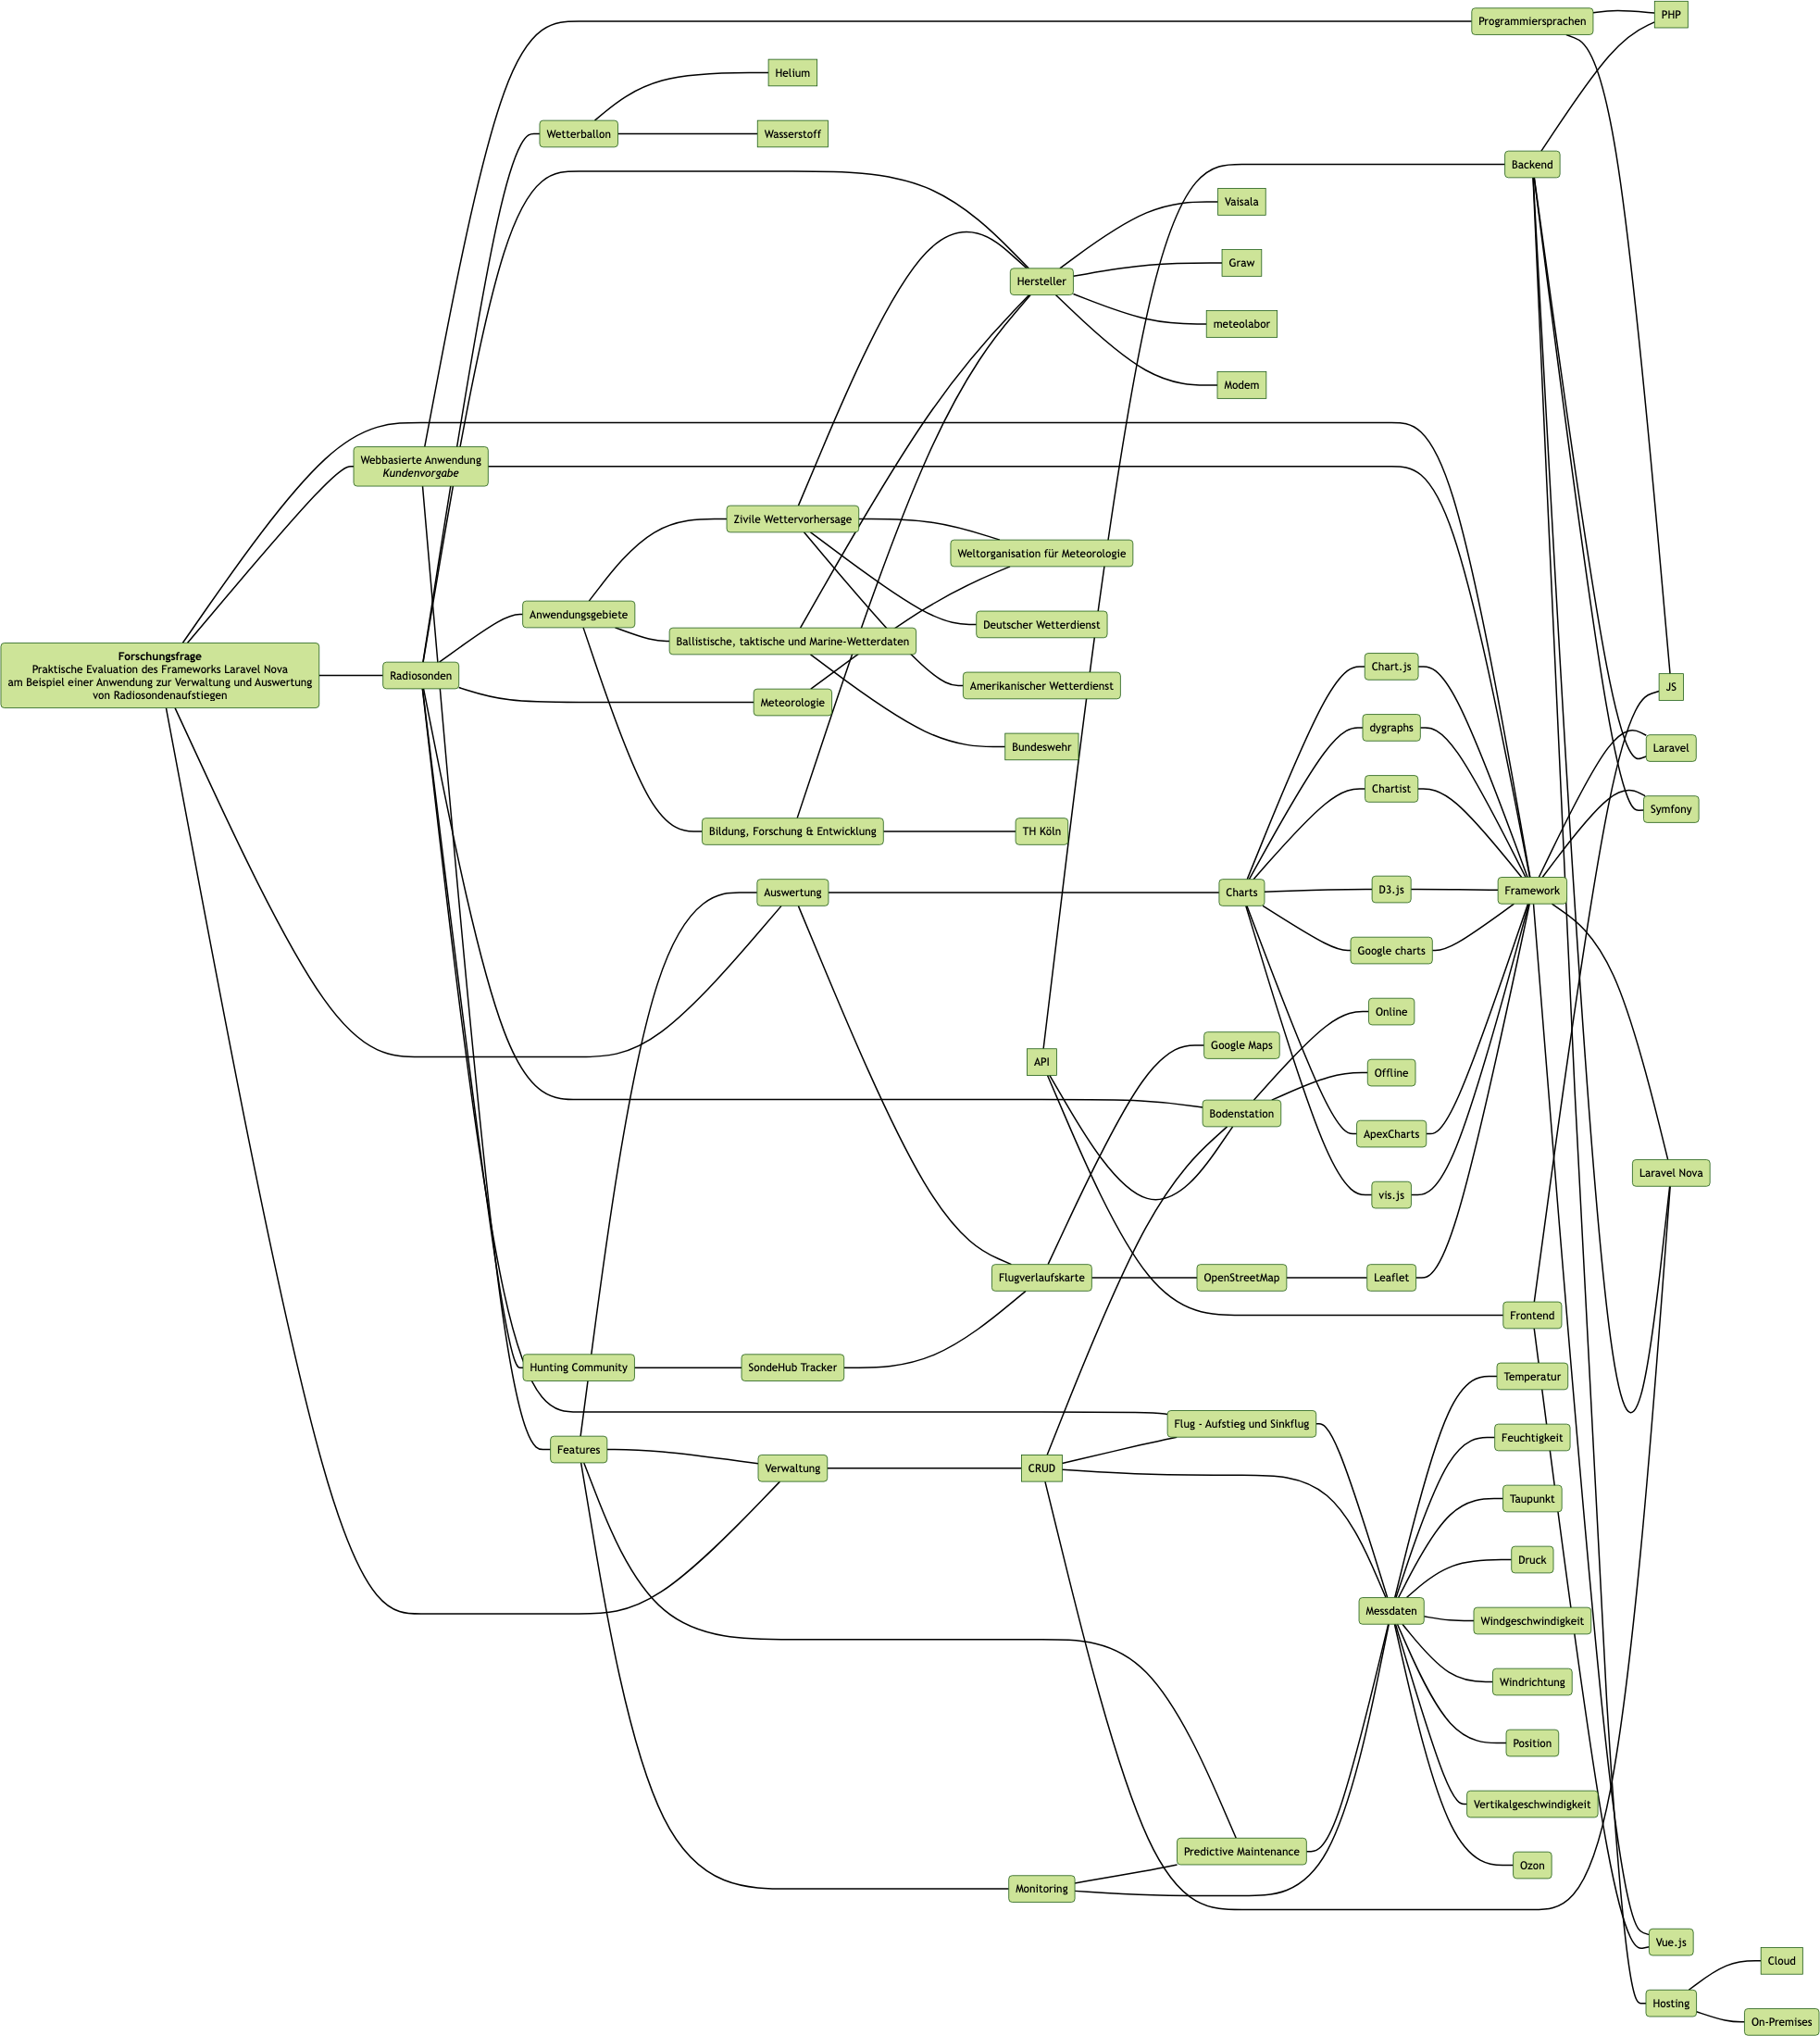
\includegraphics[scale=0.255]{assets/themenfeldanalyse_no_padding}
\end{figure}
\newpage

\section{Konzeption}
Erfahrungswerte zeigen, dass die kritischsten Technologieentscheidungen, im Bereich der Webtechnologien, das Backend betreffen, vorausgesetzt, es gibt keine speziellen Anforderungen des Frontends, die berücksichtigt werden müssen.
Daher starten die Entscheidungen im Backend und anschließend wird das Frontend festgelegt.
Auf Basis des Backends und des Frontends, sowie weiterer Projektanforderungen, wird ein passendes Hosting ausgewählt.

\subsection{Backend}

\subsubsection{PHP}
Die Entscheidung für PHP, als primäre Sprache im Backend, fiel aus zwei Gründen.
Zum einen ist PHP im Web nach wie vor ein etablierter Standard, zum anderen besteht die größte Erfahrung beim Hauptentwickler.

\subsubsection{Laravel}
Laravel ist der aktuelle Industriestandard für moderne PHP Anwendungen und dadurch die erste Wahl.
Außerdem handelt es sich bei Laravel um ein sogenanntes \enquote{batteries included} Framework, es können also verschiedene fertige Komponenten verwendet werden.
Dadurch kann schnell ein hoher Qualitätsstandard erreicht werden.

Weitere Argumente liegen in der großen Community, der guten Dokumentation und vorhandene Projekterfahrung mit dem Framework, bei vergleichbaren Projekten.

\subsubsection{Relationale Datenbank}
Die zu speichernden Daten lassen sich gut relational modellieren.
Zudem unterstützt Laravel primär relationale Datenbanken.
Das DBMS (Datenbank-Managementsystem) MariaDB überzeugt durch Open Source und die kostenlose Nutzbarkeit.
PostgreSQL als DBMS wäre eine Alternative, für und gegen die es aktuell keine weiteren Abwägungen gibt.
Die Entscheidung ist vorerst nicht kritisch für das Projekt selbst, da Datenbankanfragen nur durch einen ORM laufen, und dadurch vollständig abstrahiert sind.
\newpage

\subsection{Frontend}

\subsubsection{Chart.js}
Bisherige Projekterfahrungen seitens des Auftragnehmers zeigten Probleme mit \enquote{Google Charts}.
Gute Erfahrungen wurden hingegen mit \enquote{Chart.js} gemacht.
Die Library überzeugte in vergangen Projekten durch eine gute Dokumentation, genügend Funktionen für übliche Auswertungsarten und ein ansprechendes Design.
Als umfangreichere Library, die mehr Kontrolle bietet, ist an dieser Stelle noch \enquote{D3.js} zu erwähnen.
Um die Umsetzung möglichst effizient zu gestalten, wird auf Chart.js gesetzt.

\subsubsection{Polling}
Entgegen ersten Überlegungen zum Projektstart, wurde sich im laufenden Projekt gegen WebSockets entschieden.
Diese Entscheidung ist nicht final und wird möglicherweise in Zukunft angepasst.
Für die erste Implementierung zeigte sich, dass HTTP Polling ausreichend schnell ist, da keine wirklichen Echtzeitupdates des UI (User Interface) notwendig sind.
Von Vorteil ist die weniger komplexe und dadurch schnellere Implementierung, sowie eine vermutete Ressourcenschonung des Servers, da weniger Verbindungen offen gehalten werden müssen.

\subsection{Hosting}
Im Angebotsumfang sind zwei Hostingvarianten enthalten, daher sind die nachfolgend beschriebenen Varianten umgesetzt und vorbereitet.
Grundsätzlich ist beim Hosting zu beachten, dass dieses auch On Premises möglich ist, da bereits absehbar ist, dass einige Kunden dies verlangen werden

\subsubsection{Containerized}
Die besten Skalierungsmöglichkeiten bieten containerbasierte Anwendungen, es wird der Industriestandard Docker verwendet.
Auf Basis von Terraform, einem IaC (Infrastructure as Code) Tool, ist eine komplette Landschaft definiert.
Nach der Anbindung eines Kubernetes Clusters kann, mit einem CLI Befehl, das Hosting einer Test- und einer Produktivumgebung erstellt werden und bei Bedarf verändert werden.
Ebenfalls sind automatische Updates, durch das Bauen neuer Images und anschließende Rolling Updates, in der CI Pipeline bei GitLab implementiert.

Eine nützliche Vorarbeit für ein späteres On-Premise Hosting, ist die Entwicklung der Dockerimages.
So kann mit wenig Zusatzaufwand, auch auf lokaler Infrastruktur ein Hosting umgesetzt werden.
\newpage

\subsubsection{vServer}
Ein klassischeres Hosting hat sich im Projektverlauf als unkomplizierter gezeigt.
Ein vServer ist durch einen Entwickler selbst schnell und übersichtlich verwaltbar.
Die Komplexität eines Clusters und der damit verbundene zusätzliche Administrationsaufwand entfällt.

Außerdem gibt es keinen Overhead durch Container, man erhält die volle Leistung der gebuchten Ressourcen, dies spart langfristig Kosten.

\paragraph{Laravel Forge}
Durch den Einsatz von Laravel bietet sich die Verwendung von \enquote{Laravel Forge}\cite{laravel-forge}, einem First Party Server Management Tool, an.
Im aktuellen Projekt ergaben sich durch die Nutzung von Forge vor allem folgende Vorteile:
\begin{itemize}
    \item ein moderner und robuster Hosting Stack wird automatisiert verwaltet
    \item Push To Deploy ermöglicht schnelle Updates in Test- und Produktivsysteme
    \item automatisiert eingebundene TLS Zertifikate mittels LetsEncrypt
    \item Task Scheduling: Übersichtliche und schnelle Konfiguration durch Entwickler möglich
    \item Log File Access: gesammelter Zugriff auf alle relevanten Logfiles inklusive \enquote{Log Tailing}
\end{itemize}

Zukünftig können folgende Features von Vorteil sein:
\begin{itemize}
    \item Automatisierte Datenbankbackups
    \item Laravel Octane Support - neues Paradigma durch Stateful Server und dadurch schnellere Application Performance\cite{laravel-octane}
\end{itemize}

Als Hostinganbieter unterstützt Forge, DigitalOcean, Linode Cloud, AWS, Vultr und Hetzner Cloud.

\paragraph{Hetzner Cloud}
Die Wahl auf die Hetzner Cloud als Hostingprovider fiel eindeutig durch mehrere Vorteile:
\begin{itemize}
    \item schnelles Up- und Downscaling möglich - von einer CPU mit 2 GB RAM hoch bis auf 16 CPUs und 32 GB RAM
    \item automatisierte Backups des ganzen Servers für kleinen Aufpreis möglich
    \item günstige Preise gegenüber den anderen Anbietern
    \item Datenschutz durch Rechenzentren in Deutschland
    \item örtliche Nähe des Rechenzentrums zu GRAW - beides in Nürnberg
\end{itemize}


    \section{Durchführung}

\subsection{Technische Umsetzung}

\subsubsection{Beschreibung der entwickelten Software}

Die Anwendung ist durch einen Login geschützt und das visuelle Interface responsive umgesetzt.
Die meiste Nutzung wird am Desktop stattfinden, daher ist die UI auch hauptsächlich darauf ausgelegt.
Das Design wird durch Nova vorgegeben und ist modern.
Die verwendeten Farben und das Logo wurden auf GRAW angepasst.

\paragraph{Dashboard}
Nutzer bekommen einen Überblick über den Status von Stationen.
Aktuelle Flüge und deren Status sowie Messdaten werden in einer Tabelle und auf einer Karte dargestellt.
Die Anwendung prüft in kurzen Intervallen die Datenbank auf neue Daten und aktualisiert bei Bedarf automatisch die UI.

\paragraph{Stations}
Stationen werden auf einer Karte und als Liste dargestellt.
Innerhalb einer Station wird das Dashboard dieser Station, sowie durchschnittliche Flugstatistiken dargestellt.
Außerdem können Stammdaten editiert, Nutzer zugeordnet und Flüge ausgewählt werden.

\paragraph{Flights}
In einem Flug unterscheidet sich die Ansicht je nach Status.
Laufende Flüge zeigen den aktuellen Flugverlauf und aktuelle Daten.
Abgeschlossene Flüge zeigen Performancekriterien, thermodynamische Diagramme und Messwertdiagramme nach Zeit und Höhe.

\paragraph{Users}
Systemadministratoren können neue Nutzer erstellen und deren Rolle festlegen.
Stationsadministratoren können für ihre verwalteten Stationen Nutzer erstellen.

\newpage

\paragraph{API}
Für die native Anwendung wird eine REST Schnittstelle (\ref{fig:api}) bereitgestellt.

\begin{figure}[h!]
    \centering
    \caption{API}
    \label{fig:api}
    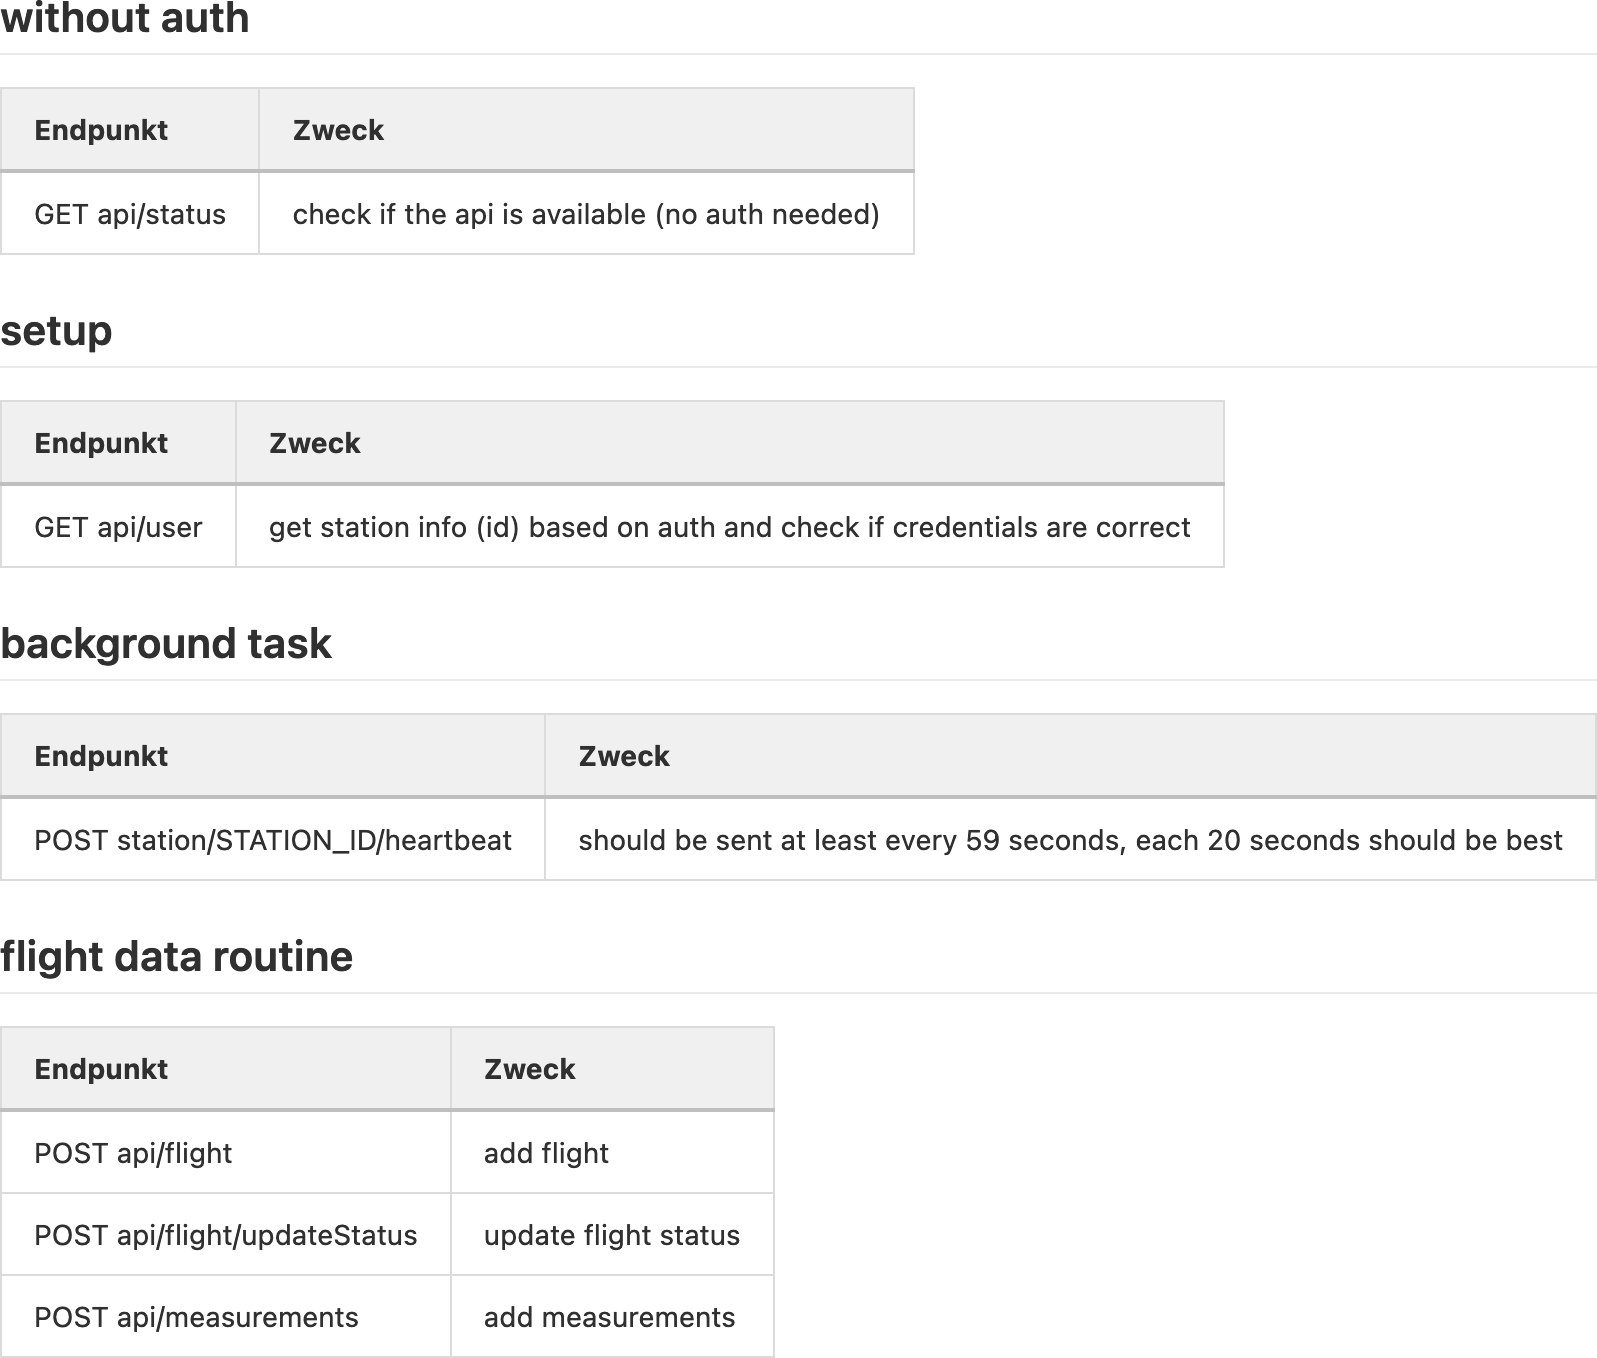
\includegraphics[scale=0.55]{assets/api}
\end{figure}
\newpage

\subsubsection{Probleme und Lösungen}

\paragraph{Verlassene Library}
Es gibt einen Fehler in der JSON Schema PHP Library, dieser wurde beim manuellen Testen der entwickelten API mit unterschiedlichen Werten gefunden.
Für die Problematik wurde folgender Issue erstellt: https://github.com/opis/json-schema/issues/123

Die Aktivität im Repository lässt allerdings vermuten, dass dieses Projekt verlassen ist.
Daher wurde vorerst die fehlerhafte \enquote{multipleOf} Validierung entfernt.
Vermutlich muss zukünftig eine andere Bibliothek gefunden werden, welche die notwendigen JSON Schema Regeln korrekt implementiert.

\paragraph{Styling von Custom Components}
Im Projekt werden viele individuelle Komponenten verwendet, um die UX der Software in Nova möglichst stark zu optimieren.
Dafür werden teilweise Komponenten wie Tabellen und Überschriften benötigt, die Nova bereits selbst implementiert.
Nova bietet es offiziell nicht an, allerdings wurde eine Lösung gefunden, wie man alle Vue Single File Components von Nova auch in den individuellen Komponenten nutzen kann.
Es muss lediglich aus der individuellen Komponente heraus ein langer relativer Pfad, bis in das Nova-Quellverzeichnis, angegeben werden.
Danach können die Komponenten gebaut und genutzt werden.

Möglicherweise gibt es zukünftig Breaking Changes seitens Nova, da dieser Import eigentlich nicht vorgesehen ist.
Dies muss bei Updates beachtet und gegebenenfalls angepasst werden.

\paragraph{Infinite Loading Tables}
Laravel Nova unterstützt neben paginated Tabellen auch ein \enquote{Load more} Pattern.
Im Projekt wurde allerdings ein \enquote{Infinite Loading} Pattern priorisiert, um eine ähnliche UX wie die native Windows Anwendung zu bieten.
Da die Tabellenkomponente von Nova selbst nicht verändert werden kann, erweitert ein separates Skript, mittels Observer Pattern, die Komponente um diese Funktion.
Alternativ könnte eine individuelle Komponente gebaut werden, dies würde allerdings zu viele Basisfeatures von Nova entfernen.
Hier zeigt sich ein Problem in der Anpassbarkeit von Nova Anwendungen, im konkreten Fall allerdings ein lösbares.

\paragraph{Kartenkomponente}
Ursprünglich sollte als Kartenkomponente das Projekt sondehub-tracker (\cite{sondehub-tracker}), bzw.\ Teile davon, eingebunden werden.
Bei genauerer Betrachtung fällt jedoch auf, dass dieses Projekt nicht als Library gebaut oder nutzbar ist.
Daher wurde es lediglich kurz analysiert und daraus die Entscheidung getroffen, die Library \enquote{Leaflet} zu nutzen.
Unter Einsatz dieser Library konnte eine interaktive Kartenkomponente entwickelt werden, welche Flüge, Stationen und Messwerte darstellt.

\paragraph{Thermodynamische Diagramme}
Im Projekt sondehub-tracker (\cite{sondehub-tracker}) gibt es ein fertiges Skew-T Diagramm.
Allerdings ist dies nur eine Projektkomponente und keine Library, und damit liegt die gleiche Problematik wie bei der Kartenkomponente vor.
Alternativ wurde bei einer weiteren Recherche jedoch die Library meteoJS gefunden.

Eine fehlende Dokumentation macht es leider notwendig, die vorhandenen Beispielimplementierungen zu analysieren und auf Basis dessen, die Komponente anzubinden.
Ebenfalls fehlt in dieser Library eine Legende, daher muss der Quellcode und die darin enthaltenen mathematischen Formeln analysiert werden, um die meteorologischen Messgrößen zu bestimmen.
Die Hürden sind überwunden und die Komponente ist funktionsfähig eingebunden.

\paragraph{Tabellensortierung}
Nova erlaubt Nutzern die Sortierung von Tabellen nach einer Spalte und als Entwickler kann man auch den zugrundeliegenden Query bereits sortieren.
Allerdings kann keine Standardsortierung nach einer Spalte konfiguriert werden.
Diese Einschränkung bei Messwerttabellen muss fürs Erste so hingenommen werden.
Bei stärker priorisiertem Bedarf, kann die Standardtabelle, durch eine individuelle Komponente, ausgetauscht werden.

\subsection{Nutzwertanalyse einiger Laravel Admin Panels}

\subsubsection{Entscheidungsproblem}
Welches Laravel Admin Panel ist für das Projekt der Sounding Console am geeignetsten?

\subsubsection{Auswahl der Entscheidungsalternativen}
Die populärsten Lösungen werden auf Basis eines Artikels ausgewählt, in dem sich eine Alternative selbst mit Anderen vergleich (Siehe~\cite{the-guide-to-laravel-admin-panels}).
Es ist davon auszugehen, dass ein Anbieter in diesem Bereich, die eigene Konkurrenz gut kennt.

\subsubsection{Bestimmung der Entscheidungskriterien}
TODO

BASIS: https://blog.forestadmin.com/the-guide-to-laravel-admin-panels

genug Ressourcen für Individualentwicklung

Konfiguration durch technisch weniger versierte Personen; also Low Code

Projektziel: MVP oder skalierbare Architektur

ERWEITERN durch eigene kriterien:

Lizenzmodell

Preis im MVP Projekt

Preis über Produktlaufzeit

Anpassbarkeit

Flexibles Hosting

\subsubsection{Gewichtung der Entscheidungskriterien}
TODO

\subsubsection{Bewertung der Entscheidungskriterien}
Laravel Nova
https://nova.laravel.com
rapid dev time, good structure, extensible through components

Filament
https://filamentphp.com/

Backpack
https://backpackforlaravel.com/

Voyager
https://voyager.devdojo.com/

Quick Admin Panel
https://quickadminpanel.com/

Einmalige Code Generierung
alter Stack (jQuery); neuere Stacks (Vue.js oder Tailwind) noch Beta und wenige Features
viele Freiheiten nach erster Erstellung, dafür dann auch langsamer

Forest Admin
https://www.forestadmin.com/
SAAS
Low Code (z.B. UI Layout Editor)

\subsubsection{Berechnung des Nutzwerts/Scores}
TODO

    \section{Reflektion}

\subsection{Kommunikation}
Die Kommunikation bezüglich der Anforderungen zwischen Auftraggeber und Entwickler verlief schnell und zielorientiert.
Das anhand dieser Absprachen entwickelte und verschriftlichte Leistungspaket, ermöglichte eine stringente Implementierung.

Die Kommunikation bezüglich der Schnittstellen zu GRAWMET verlief inhaltlich gut, durch sehr begrenzte Entwicklungsressourcen beim Auftraggeber allerdings eher langsam.
Daher ist bisher nur die Anbindung für laufende Flüge implementiert, jedoch nicht der Import alter Flüge.
Dieser wurde zeitlich nicht priorisiert und bleibt daher, aufgrund fehlender Informationen zu bestehenden Datenformaten, vorerst offen.

Trotz guten und sehr konkreten Absprachen bezüglich der Bodenstationen, stellte sich erst im späteren Projektverlauf heraus, dass es auch bewegliche Bodenstationen gibt.
Durch die Abwesenheit von Produktivdaten konnte jedoch schnell das Schema angepasst werden und eine 1:n-Beziehung, zu einer neuen Positionsressource, implementiert werden.

\subsection{Zielerreichung}
Das grundsätzliche Projektziel wurde vollständig erreicht.
Die entwickelte Sounding Console ist voll funktionsfähig und verhält sich, in der generellen Benutzererfahrung, vergleichbar zu ausgereiften Applikationen.
Das Interface reagiert schnell auf Benutzereingaben und ist grundsätzlich verständlich.

Der geplante Funktionsumfang wurde, bis auf wenige Ausnahmen, vollständig abgedeckt.
Teilweise wurden sogar Features implementiert, die im Funktionsumfang nicht, oder nur optional, vorgesehen waren.

    \section{Fazit und Ausblick}

\subsection{Beantwortung der Projektfragen}

\textbf{\enquote{Welche Vor- und Nachteile bietet der Einsatz eines Admin Panels am konkreten Beispiel von Laravel Nova?}}\\
Die Aussage von Elson Tan \enquote{Great to get started, hard to customise later on}(\cite{laravel-nova-in-production-one-year-later}) fasst die Problematik gut zusammen.
Laravel Nova ermöglicht insbesondere Aufgaben im Bereich der Datenverwaltung sehr effizient.
Individuelle Anforderungen umzusetzen, benötigt allerdings verhältnismäßig viel Zeit.

\textbf{\enquote{Lässt sich die Sounding Console grundsätzlich mit Nova umsetzen, oder gibt es zu starke Einschränkungen bei der Umsetzung der Anforderungen?}}\\
Ja, für die Erprobung eines MVP ist Nova im Fall der Sounding Console gut geeignet, allerdings werden zukünftige Anforderungen zeigen, ob eine komplett individuelle, und damit auch besser anpassbare, Lösung der bessere Weg ist.

\textbf{\enquote{Welche Anforderungen der Sounding Console lassen sich durch Nova besonders gut entwickeln?}}\\
Datenverwaltung und einfache Metriken.

\textbf{\enquote{Bei welchen Anforderungen entstehen Nachteile durch die Verwendung von Nova?}}\\
Individuelle UX und UI Anforderungen bringen Nova an die Grenzen des Machbaren.

\textbf{\enquote{Lässt sich abschätzen, ob zukünftige Erweiterungen gut mit Nova umsetzbar sind?}}\\
Grundsätzlich können noch einige Erweiterungen sinnvoll mit Nova gebaut werden, allerdings wird die Software vermutlich mit wachsenden Funktionen irgendwann schlechter Benutzbar, da der Spielraum für UI-Anpassungen stark begrenzt ist.

\textbf{\enquote{Können am vorliegenden Beispiel Muster erkannt werden, welche Anforderungsbereiche betroffen sind, um auf Basis dessen zukünftige Projektentscheidungen zu treffen?}}\\
Ja, sobald ein Projekt größer oder individueller ist, sollte eine offenere Architektur gewählt werden.

\textbf{\enquote{Wie flexibel ist der Technologie Stack und wie sehr wird man durch Nova eingeschränkt?}}\\
Der Technologie Stack ist eingeschränkt, ebenso sind es Entwickler bei der Wahl der Lösungen, vor allem im Frontend.
Die individuellen Komponenten ermöglichen viel, sobald es aber um den generellen Aufbau des Systems und um ganze Seitenlayouts geht, stößt Nova an Grenzen.

\subsection{Fazit}
Die Verwendung von Nova war in diesem Praxisprojekt insgesamt von Vorteil.
Die Architektur ist im Backend flexibel und könnte durch ein neues Frontend ergänzt werden.
Dabei könnten auch die individuellen Komponenten wiederverwendet werden und die Struktur der aktuellen Anwendung grundsätzlich nachgebaut werden.

Das Ergebnis der Arbeit ist nicht wirklich überraschend.
Frameworks, insbesondere opinionated Frameworks wie Nova, bieten viel und schränken dadurch auch ein.
Dessen sollte man sich bewusst sein und dies im technischen Entscheidungsprozess berücksichtigen.

\subsection{Ausblick}
Die entwickelte Software soll zeitnah bei Messnetzwerken in den produktiven Betrieb gehen.
Zuvor werden noch einige interne manuelle Tests durchgeführt und verschiedene Optimierungen an der Software umgesetzt.
Erste potenzielle Baustellen für Optimierungen wurden bereits durch Testläufe entdeckt.

Zusätzlich sollen realistische Lasttests entwickelt werden, um die Performance der Software bereits vor dem echten Betrieb zu testen.
Dadurch wird sich auch zeigen, welche Leistung das Hosting zu Spitzenzeiten abdecken können muss.

Ebenso soll die umgesetzte Architektur geprüft werden und gegebenenfalls vor der Markteinführung überarbeitet werden, sofern eine Analyse dafür Notwendigkeiten zeigt.
Dieser Arbeitsschritt soll möglicherweise im Rahmen einer, auf diesem Praxisprojekt aufbauenden, Bachelorarbeit stattfinden.


    \appendix

% Quellenverzeichnis
\newpage


\section{Quellenverzeichnis}
\bibliographystyle{plain}
\printbibliography

% Abbildungsverzeichnis
\newpage
\renewcommand{\listfigurename}{Abbildungsverzeichnis}
\listoffigures

% Tabellenverzeichnis
\renewcommand{\listfigurename}{Tabellenverzeichnis}
\listoftables

% Anhang
\newpage


\section{Anhang}

\subsection{Eigenständigkeitserklärung}
%\frame{\includegraphics[scale=0.183]{assets/eigenstaendigkeitserklaerung}}

\subsection{Leistungspaket}\label{subsec:leistungspaket}
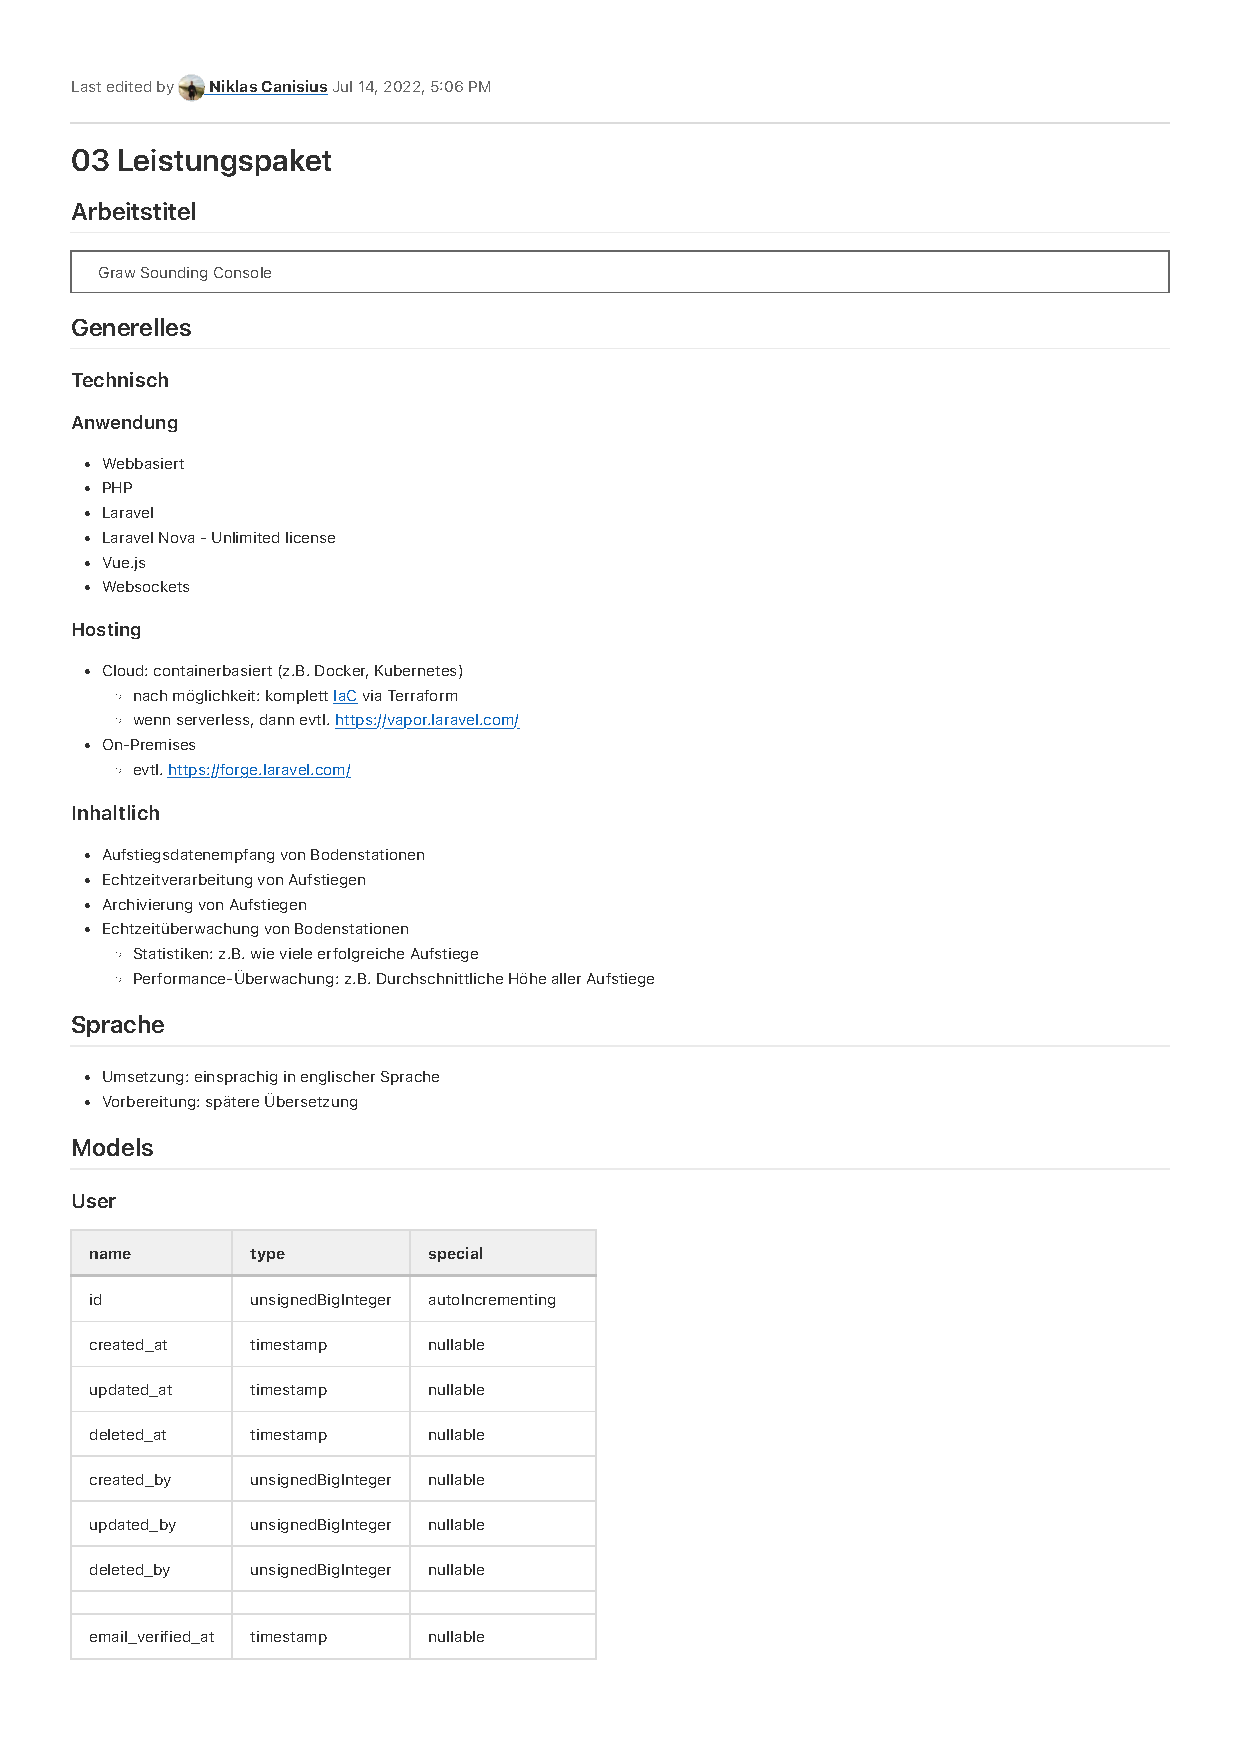
\includepdf[pages=-]{assets/Leistungspaket.pdf}

\subsection{Angebot}\label{subsec:angebot}
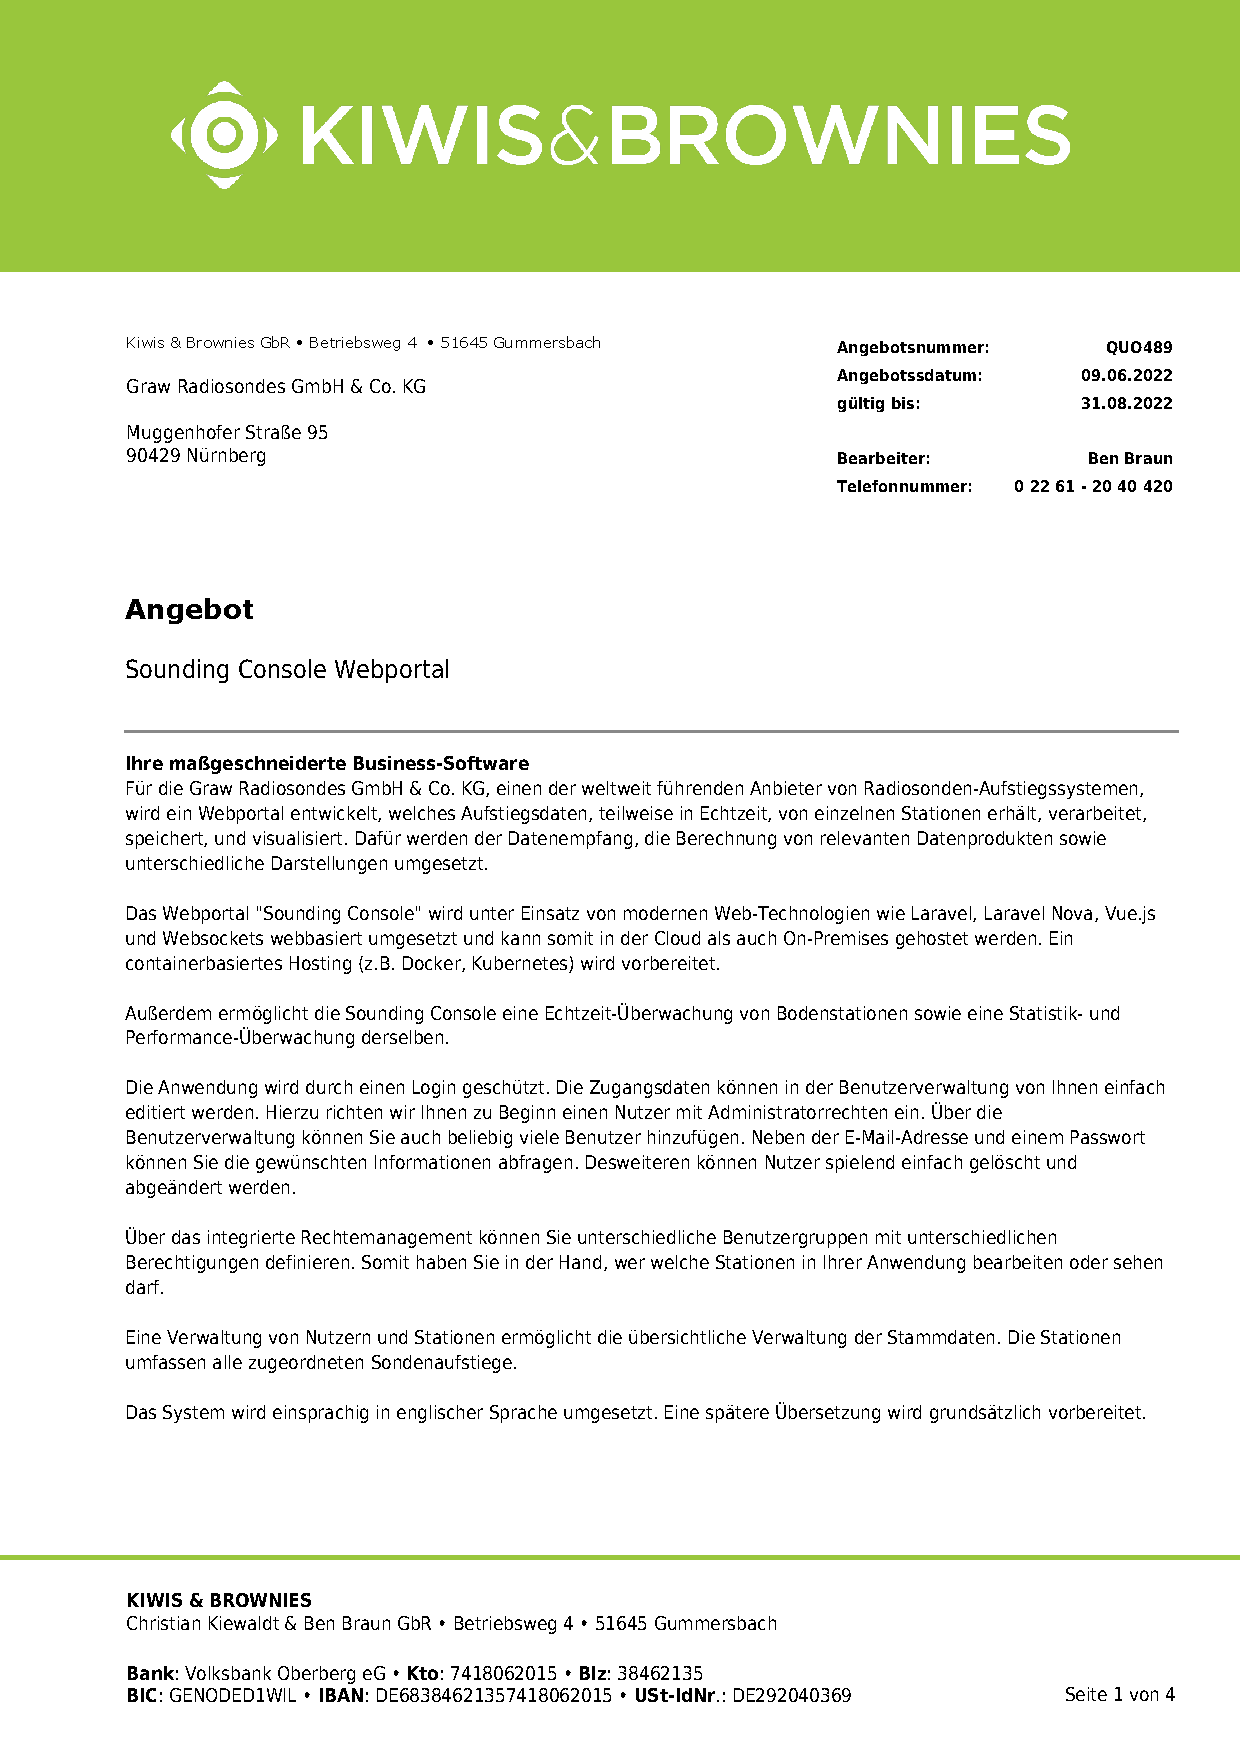
\includepdf[pages=-]{assets/Angebot.pdf}

\subsection{Lastenheft}\label{subsec:lastenheft}
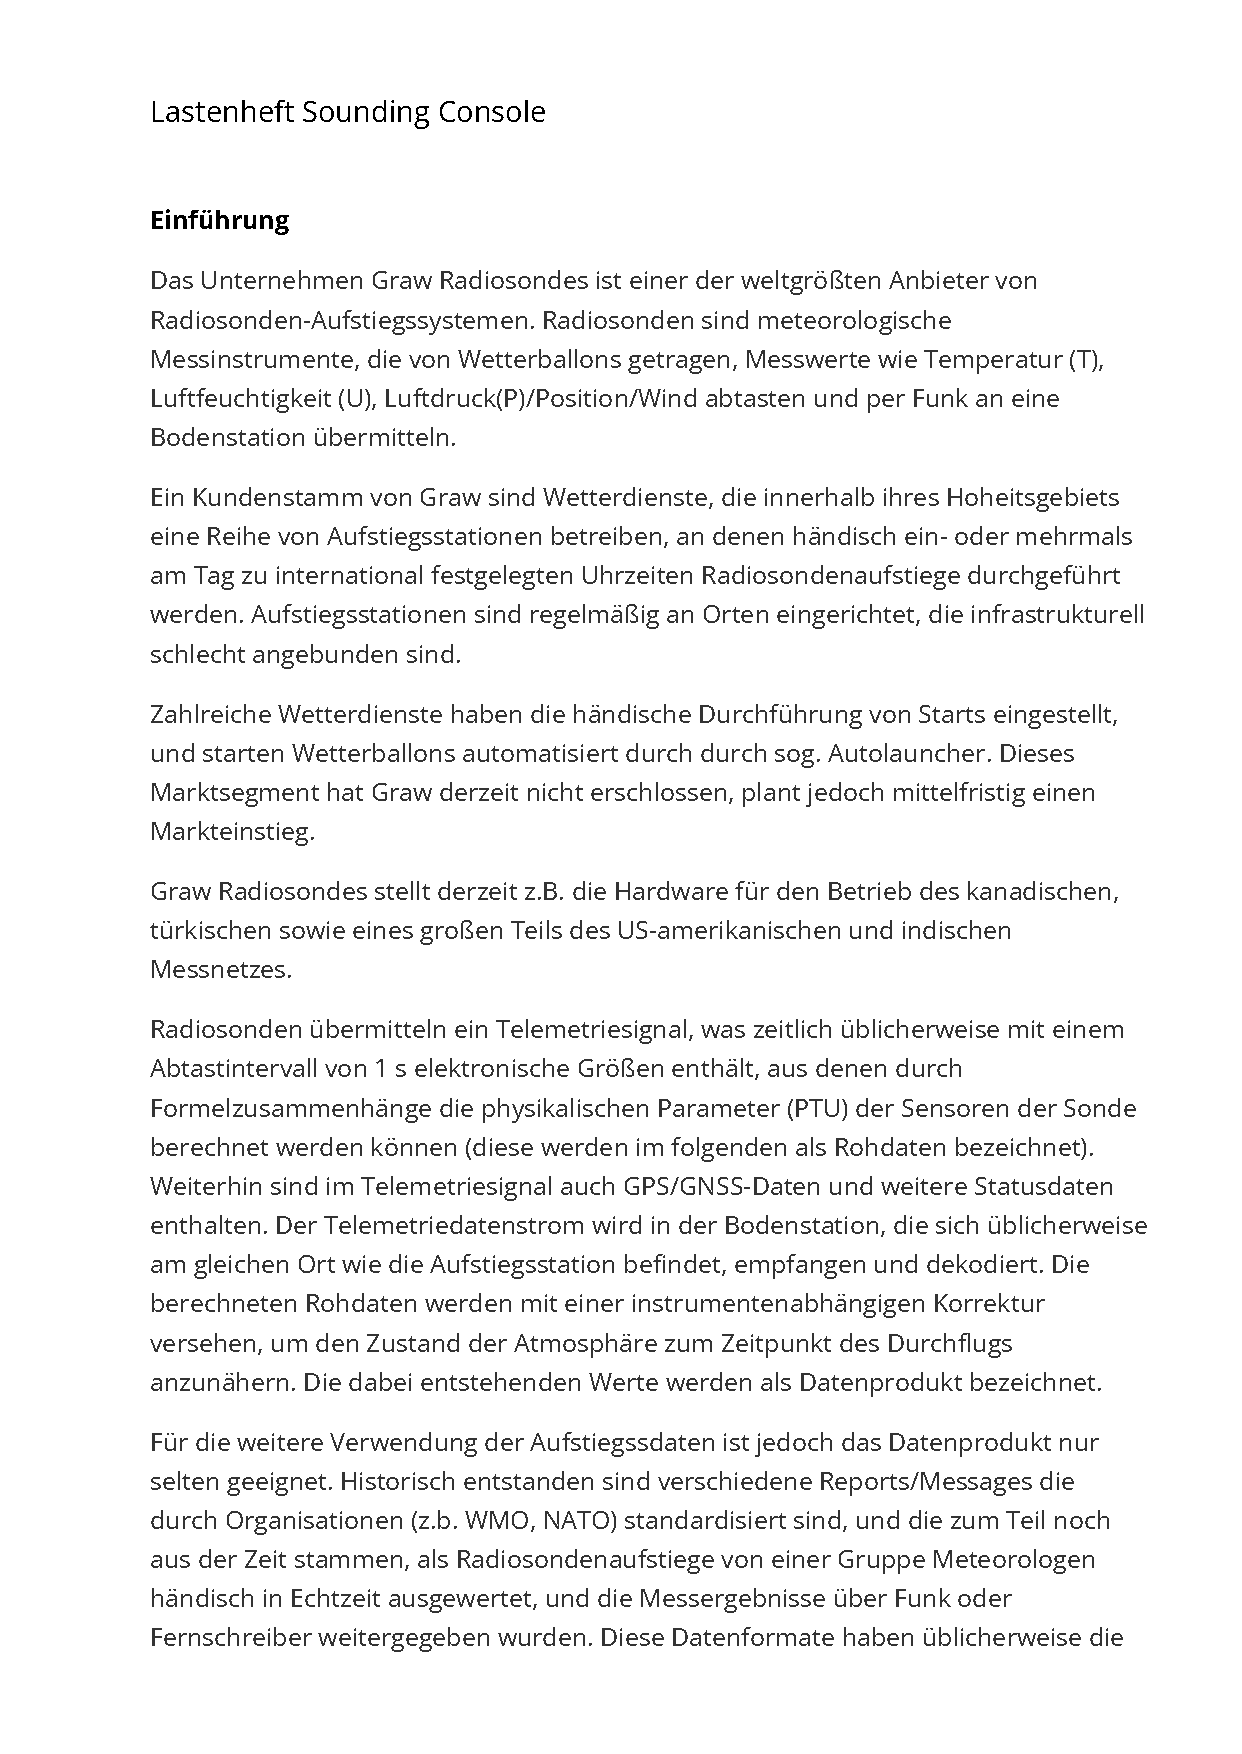
\includepdf[pages=-]{assets/Lastenheft.pdf}

\end{document}
